\documentclass[11.5pt]{sig-alternate} % sets document style to sig-alternate
% packages
% typesetting
%\usepackage{dirtytalk} % typset quotations easier (\say{stuff})
\usepackage{hanging} % hanging paragraphs
\usepackage[defaultlines=3,all]{nowidow} % avoid widows
\usepackage[pdfpagelabels=false]{hyperref} % produce hypertext links, includes backref and nameref
\usepackage{xurl} % defines url linebreaks, loads url package
\usepackage{microtype}
%\usepackage{textcomp}
%\newcommand{\texttildemid}{\raisebox{0.4ex}{\texttildelow}}
% layout
\usepackage{enumitem} % control layout of itemize, enumerate, description
\usepackage{fancyhdr} % control page headers and footers
\usepackage{float} % improved interface for floating objects
%\usepackage{multicol} % intermix single and multiple column pages
% language
\usepackage[utf8]{inputenc} % accept different input encodings
\usepackage[english]{babel} % multilanguage support
% misc
\usepackage{graphicx} % builds upon graphics package, \includegraphics
%\usepackage{lastpage} % reference number of pages
%\usepackage{comment} % exclude portions of text (?)
\usepackage[table]{xcolor} % color extensions
\usepackage[backend=biber, style=apa]{biblatex} % sophisticated bibliographies % necessary for HTML to display author info and date on abstract page
\usepackage{csquotes} % advanced quotations, makes biblatex happy
\usepackage{authblk} % support for footnote style author/affiliation
% tables and figures
\usepackage{tabularray}
%\usepackage{array} % extend array and tabular environments
\usepackage{caption} % customize captions in figures and tables (rotating captions, sideways captions, etc)
%\usepackage{cuted} % allow mixing of \onecolumn and \twocolumn on same page
\usepackage{multirow} % create tabular cells spanning multiple rows
%\usepackage{subfigure} % deprecated, support for manipulation of small figures
%\usepackage{tabularx} % extension of tabular with column designator "x", creates paragraph-like column whose width automatically expands
%\usepackage{wrapfig} % allows figures or tables to have text wrapped around them
%\usepackage{booktabs} % better rules
% dummy text
%\usepackage{blindtext} % blind text dummy text
%\usepackage{kantlipsum} % Kant style dummy text
\usepackage{lipsum} %lorem ipsum dummy text
% other helpful packages may be booktabs, longtable, longtabu, microtype

\pagestyle{fancy} % sets pagestyle to fancy for fancy headers and footers

% header and footer
% modern way to set header image
\renewcommand{\headrulewidth}{0pt} % defines thickness of line under header
\renewcommand{\footrulewidth}{0pt} % defines thickness of line above header
\setlength\headheight{80.0pt} % sets height between top margin and header image, effectively moves page contents down
\addtolength{\textheight}{-80.0pt} % seems to affect the lower height. maybe only works properly if footer numbers enabled?
\fancyhf{}
\fancyhead[CE, CO]{
\includegraphics[width=\textwidth]{headerImage.png}}
% footer
%\fancyfoot[LE,LO]{Article Title Here \\ DOI: }% left footer article title and doi
%\fancyfoot[CE,CO]{{}} % center footer empty
%\fancyfoot[RE,RO]{\thepage} % right footer page numbers
%\pagenumbering{arabic} % arabic (1, 2, 3) numbering in footer

\hypersetup{colorlinks=true,urlcolor=blue} % sets link color to blue
\urlstyle{same} % sets url typeface to same as rest of text

% set caption and figure to italics, label bold, left align captions, does not transfer to HTML
\captionsetup{labelfont=bf, font={large, it}, justification=raggedright, singlelinecheck=false}
\renewcommand\theContinuedFloat{\alph{ContinuedFloat}}

%this next bit is confusing, but essentially changes the width of the abstract. Seems to have been copied from this https://tex.stackexchange.com/questions/151583/how-to-adjust-the-width-of-abstract
\let\oldabstract\abstract
\let\oldendabstract\endabstract
\makeatletter %changes @ catcode to enable modification (in parsep)
\renewenvironment{abstract} %alters the abstract environment
{\renewenvironment{quotation}%
               {\list{}{\addtolength{\leftmargin}{1em} % change this value to add or remove length to the the default ?
                        \listparindent 1.5em%
                        \itemindent    \listparindent%
                        \rightmargin   \leftmargin%
                        \parsep        \z@ \@plus\p@}%
                \item\relax}%
               {\endlist}%
\oldabstract}
{\oldendabstract}
\makeatother %changes @ catcode to disable modification

% checks
% italics-
% links -
% dashes
% tildes -
\begin{document}

\title{Making Science Accessible to Students with \\ Significant Cognitive Disabilities}

\author[1]{\large \color{blue}Lori Andersen}
\author[1]{\large \color{blue}Brooke Nash}

\affil[1]{University of Kansas}

\toappear{}
%% ABSTRACT
\maketitle
\begin{@twocolumnfalse} 
\begin{abstract}
\item 
\textit{The publication of A Framework for K-12 Science Education (National Research Council, 2012) and the Next Generation Science Standards (NGSS Lead States, 2013) have created a need for new alternate content standards and alternate assessments in science that are linked to the new general education science standards. This article describes how a consortium of four states used Evidence-Centered Design (Mislevy, Steinberg,\& Almond, 2003) and Universal Design for Learning (CAST, 2012) to develop alternate science content standards and assessments. A set of 43 alternate science content standards was created and an alternate assessment at each of three grade spans. Evidence that supports appropriateness of the alternate standards for students with SCD and fidelity of representation of the Framework is presented. One cycle of testlet/item development was conducted. Results of a pilot test (251 items; 1,606 students) are presented. Evidence for validity and accessibility of the alternate assessment is presented. Major findings include that the assessment items met accessibility, bias and sensitivity, and content requirements, and that students were able to understand and respond to assessment items. Data from a pilot assessment provided evidence of the accessibility of the standards and assessments. The implications of this work for teaching science to students with SCD and preliminary efforts to develop supports for teachers are discussed.}
\\ \\
Keywords: students with significant cognitive disabilities, NGSS, alternate assessment
\end{abstract}
\end{@twocolumnfalse}

%% AUTHOR INFORMATION

\textbf{*Corresponding Author, Lori Andersen}\\
\href{mailto:  landersen@ku.edu}{(landersen@ku.edu)} \\
\textit{Submitted  Jan 15 2016 }\\
\textit{Accepted May 16 2016} \\
\textit{Published online Jun 13 2016} \\
\textit{DOI: 10.14448/jsesd.09.0002} \\
\pagebreak
\clearpage
\begin{large}
   
\section*{INTRODUCTION}

Little research exists regarding how students with significant cognitive disabilities (SCD) learn or understand science concepts (Browder et al., 2012, Courtade, Spooner,\& Browder, 2007), even though science content that is linked to grade-level, general education science standards has been mandated for these students since 2004 (Individuals With Disabilities Education Improvement Act [IDEIA], 2004). Limited expectations have been observed in the enacted science curriculum for students with SCD (Karvonen et al., 2011) and in the methods used for science instruction (e.g, Browder et al., 2014). Science content for students with SCD has focused on life skills rather than science concepts, and science instructional methods are based on behavioral changes rather cognitive development (e.g,, Browder et al., 2014; Spooner et al., 2012). As a result, students with SCD have typically been provided science content that is more appropriate for much younger students instead of content that is age appropriate (Karvonen et al., 2011). Solving the problem of making science accessible to students with SCD will require changes to both teaching and assessment. For example, gaining evidence of student learning in science requires reliable and valid assessments. At the same time, student learning also depends on accessible, high-quality science instruction. This paper describes new alternate science standards and alternate assessments for students with SCD, as well as the implications of these changes for science instruction. 

\section*{LITERATURE REVIEW}

Students with SCD comprise the 1\% of the K-12 student population who participate in alternate assessments based on alternate achievement standards (Federal Register, December 9, 2003). While this low-incidence population of students is highly heterogeneous, they exhibit several general characteristics: 1) They have a disability or multiple disabilities that significantly impact intellectual functioning and adaptive behavior; 2) They are primarily instructed using alternate content standards that are less complex than grade-level content standards; and 3) They require extensive direct individualized instruction and substantial supports to achieve measureable gains in the grade-and age-appropriate curriculum (Dynamic Learning Maps, 2013). Specific components of these students' cognitive architecture that pose challenges include limited working memory and long-term memory (Kleinert et al., 2009).  Such cognitive differences must be taken in to consideration in the design of standards, curriculum, and assessments to increase accessibility through Universal Design for Learning (UDL; Cast, Inc., 2012). 

Universal Design for Learning (UDL; Cast, Inc., 2012) is a model for creating instructional goals, assessments, methods and materials that are accessible to students. The model uses three factors to increase accessibility when adapting materials to learner characteristics: multiple means of engagement, multiple means of representation, and multiple means of action and expression. However, before the model can be applied the characteristics of the learners must be known. A prior census of students with SCD (n=44,782; Dynamic Learning Maps, 2013) informs this research, describing characteristics commonly found within this population. For example, the survey identified that the majority of students' reading levels were at or below the second grade level. This learner characteristic led to decisions concerning multiple means of representation to make content accessible, particularly the accessibility of text and the use of core vocabulary. Thus, a high school student can be taught and assessed on high school science concepts that are made accessible through text that is written a level that is appropriate for the students' reading levels. Knowing the characteristics of the students is critical to identifying changes that will make science assessments and instruction accessible. 

Students with significant cognitive disabilities do not participate in the same large-scale assessments as most students. Science assessments for students with SCD have included methods such as portfolios, which tend to have lower reliability and validity than more standardized assessments. Recently, large-scale science assessments for students with SCD have changed because technology has provided greater accessibility (e.g., Karvonen, Bechard,\& Wells-Moreaux, 2015). However, the cognitive characteristics and communication modalities prevalent in the population pose challenges to reliable and valid measures of conceptual understanding of science. Furthermore, the characteristics of the new science framework have increased cognitive demands for all students, including students with SCD. For assessments to be reliable and valid, accessibility features must allow students to demonstrate what they know, despite the challenges presented by their cognitive characteristics and/or communication modalities. 

Students with SCD are underrepresented in the science education research literature (Courtade et al., 2007), despite an emphasis in science education reform documents on science literacy for all students (e.g., National Science Education Standards, A Framework for K-12 Science Education). Some special education research has described how strategies that are commonly used with students with SCD could be applied in science teaching, such as task analysis (e.g., Browder et al., 2014; Spooner et al., 2012; Wakeman, Karvonen,\& Ahumada, 2014) or time delay (e.g., Browder et al., 2007). Scant research has explored the use of conceptual science teaching approaches with students with SCD. A few studies have described how students with SCD can be taught to use an inquiry model to answer science-related questions that are relevant to daily living (e.g., Miller, Doughty,\& Krockover, 2015; Miller, Krockover,\& Doughty, 2013). However, no research has explored students with SCD's conceptual understanding of science disciplinary core ideas. One problem of a focus on typical special education strategies, such as task analysis and time delay, is that these strategies are not likely to help students develop conceptual understanding. There is no empirical evidence that supports the use of methods such as task analysis and time delay to develop science conceptual knowledge. Evidence does support the use of task analysis to teach the steps of a general inquiry model that can then successfully generalized to other situations (e.g., Miller et al., 2015) and the use of time delay to teach science vocabulary (e.g., Wakeman et al., 2013). However, the \textit{Framework} demands that students will be able to demonstrate understanding of science concepts through science practices such as evidence-based argumentation or modeling (National Research Council, 2012). These understandings need to be measured with reliable and valid assessments. The present study fills this gap in the research.

The Dynamic Learning Maps™ Alternate Assessment System was developed using principles of Evidence Centered Design (ECD; Mislevy, Almond,\& Lukas, 2003) and Universal Design for Learning (Cast, Inc., 2012). The first DLM operational assessments (in ELA and math) were administered in the 2014-2015 school year. The Dynamic Learning Map Science Consortium was formed in 2014 to address the need for alternate science assessments that linked to general education science content. As the general design and accessibility features are based on research that was conducted for the DLM English language arts (ELA) and Mathematics assessments, the DLM Science Alternate Assessment builds on well-established practices (e.g., Wells-Moreaux, Bechard,\& Karvonen, 2015).

\section*{RESEARCH QUESTIONS}

The first task of the consortium was to create a common set of alternate content standards that would be the basis of the science alternate assessment. Thus, the first research question was: How can the science disciplinary core ideas, crosscutting concepts, and science and engineering practices described in \textit{A Framework for K-12 Science Education} be made accessible to students with SCD? Once alternate content standards were created, the second task was to create assessment items. The second research question was: How can the new alternate standards be assessed? A third question was: How do we know the newly created alternate standards and assessments accessible?

\section*{METHOD}

The method for the study synthesizes Evidence-Centered Design (ECD; Mislevy et al., 2003), and Universal Design for Learning (UDL, Cast Inc., 2012).     

Evidence-centered design guided decisions about what evidence would be collected to determine if specific claims have been met, while UDL guided the considerations that affect accessibility for students with SCD. Figure 1 shows how components of ECD were integrated with UDL considerations throughout the process. Each research question includes a small set of claims and evidence. A visual overview of the claims and evidence involved in each of the three research questions is provided in Figure 1. In the following section, the method used to answer each research question is described in detail. The results for each research question are presented immediately following each the description of the method for that research question. Conclusions are presented after all three sets of methods and results.

\begin{figure*}[ht]
    \centering
    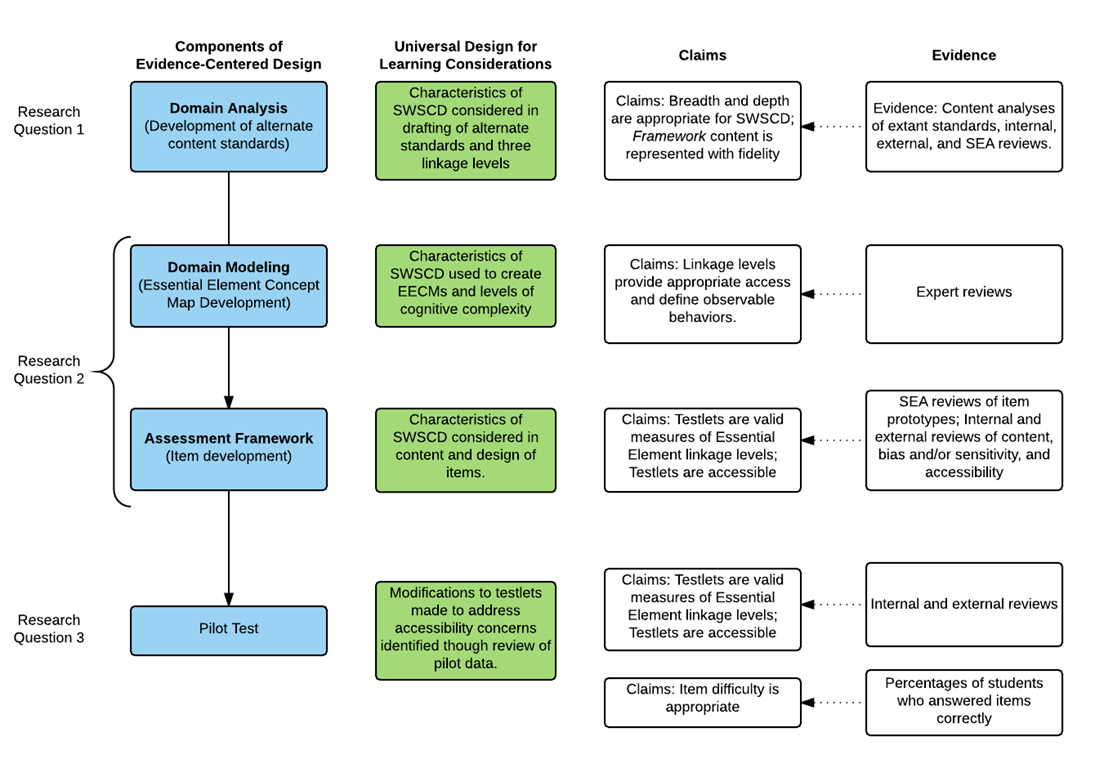
\includegraphics[width=1\linewidth]{images/fig1.png}
    \caption{Study Overview}
\end{figure*}

\subsection*{Method for Research Question 1}

A multi-step process was used to answer the first research question; the method is based on Evidence Centered Design (ECD; Mislevy et al., 2003) and Universal Design for Learning (UDL; Cast, Inc., 2012). First, common science topics were identified through content analysis of states' extant alternate science standards. This content analysis marks the beginning of the \textit{Domain Analysis} phase of ECD (Figure 1). Then, the common topics were mapped onto the \textit{Framework} Disciplinary Core Idea topics. Grade-level content within those topics was identified using the \textit{Framework} and the \textit{Next Generation Science Standards}. Alternate content standards were drafted and revised in an iterative process by various stakeholders and experts through the application of UDL principles. 

\subsection*{Results for Research Question 1}

Content of the existing alternate science standards from seven states was analyzed. Common science topics in Physical Science, Life Science, and Earth and Space Science in state alternate content standards were identified. These topics served as the starting points for new alternate content standards within these areas. Next, corresponding Disciplinary Core Idea topics in \textit{A Framework for K-12 Science Education} (National Research Council, 2012) were identified and specified by the \textit{Framework} code and name (Table 1). This content analysis allowed the breadth of the \textit{Framework} to be reduced to a subset of topics that were most relevant to students with SCD.

\begin{table*}[th]
\caption{Common Disciplinary Core Ideas (DCI) Topics in State Alternate Science Standards}
\begin{tabular}{ll}
\hline
Science Area & Common Disciplinary Core Idea Topics \\ \hline
Earth and Space Science	& ESS.1B Earth and the Solar System \\
Science & ESS.2A Earth materials and systems \\
& ESS.2D Weather and climate \\
& ESS.3A Natural resources \\
& ESS.3C Human impacts on Earth systems \\
Life Science & LS.1A Structure and function  \\
& LS.1B Growth and development of organisms \\
& LS.2A Interdependent relationships in ecosystems \\
& LS.2B Cycles of matter and energy transfer in organisms  \\
& LS.3A Inheritance of traits \\
& LS.3B Variation of traits \\
& LS.4C Adaptation \\
Physical Science & PS.1A Structure and properties of matter  \\
& PS.2A Forces \& motion,  \\
& PS.2B Types of interactions  \\
& PS.3D Energy and chemical processes in everyday life \\
& PS.4A Wave properties \\ \hline
\end{tabular}
Note: 7 states’ alternate content standards were analyzed
\end{table*}

For the purpose of the DLM Science Consortium, elementary (grade band 3-5), middle school, and high school were selected as the levels at which students would be assessed. States' alternate content standards were typically grouped into four content strands: inquiry science, life science, physical science, and earth and space science. However, the \textit{Framework} has a different structure that consists of three distinct dimensions: disciplinary core ideas, science or engineering practices, and crosscutting concepts. The disciplinary core ideas were selected based on the content analysis of extant state alternate content standards (Table 1). The crosscutting concepts were not included explicitly in the new alternate content standards because crosscutting concepts were not identified as common topics in extant alternate content standards. The science and engineering practices were targeted as learning goals even though the science and engineering practices were not explicitly represented in most states' extant science content standards. States' standards typically included scientific inquiry skills as a separate science topic. Grade-level content within the two dimensions, disciplinary core idea and science or engineering practice, was identified using the \textit{Next Generation Science Standards} and extant state alternate content standards as guides. In the next section, the process by which the alternate science content standards were drafted is described.

At each assessed grade level (5th grade, middle school, high school), corresponding grade-level \textit{Next Generation Science Standards} were identified as the links from to the general education content standards. Each alternate standard integrated a disciplinary core idea topic and a science or engineering practice. The pairings of science or engineering practices with disciplinary core ideas were based on the pairings in the \textit{Next Generation Science Standards} for the corresponding grade-level standard. In this way, the grade-level \textit{NGSS} standards provided links from the new alternate content standards to the general education standards. 

Using principles of Universal Design, one grade-level alternate science standard was crafted for each corresponding \textit{NGSS} standard. Alternate science standards are less complex and more accessible in terms of both the disciplinary core idea and the science or engineering practice. These reductions in cognitive complexity are intended to make the \textit{Framework} accessible to students with SCD. In this manner, an initial set of alternate content standards was drafted. 

A unique feature of the DLM science alternate assessment system is the use of three \textit{linkage levels} for each alternate content standard. The grade-level alternate standard is the \textit{target} linkage level. For each target, two corresponding expectations, or \textit{linkage levels}, were created that linked to the same science concept with reduced breadth, depth, and/or complexity. These two linkage levels are called the precursor linkage level and the initial linkage level. The precursor linkage level has less depth and complexity than the target linkage level. The initial linkage level has the least depth and complexity. All three linkage levels are linked to the same science Disciplinary Core Idea topic and science or engineering practice. 

The proposed standards were reviewed by a panel of experts who specialized in teaching students with SCD or science. These experts included state-level science and/or special education leaders as well as university and/or special education faculty. Through a series of four meetings, the alternate standards and linkage levels were revised to improve accessibility while still maintaining links to the grade-level content. The first draft was compiled and then reviewed internally by an expert panel of science and special education consultants, which resulted in a second draft. The second draft was presented to representatives from each state education agency and the educators and content specialists that they selected. Sixteen experts in science, as well as seventeen individuals with expertise in instruction for students with SCD from across five states reviewed the draft documents. This review resulted in significant changes that: (1) clarified science concept targets, (2) clarified statements related to the science and engineering practices, (3) better employed Universal Design principles, (4) made linkage levels more measurable, (5) better aligned the linkage levels with the grade-level standards, and (5) provided examples to clarify descriptions. A third draft was then reviewed internally by each state. A final discussion and consensus vote occurred in December 2014. The resulting alternate content standards are called the DLM Science Essential Elements (Dynamic Learning Maps, 2015).

Table 2 shows an Essential Element (EE) from the elementary school grade span. The \textit{NGSS} standard was used to identify the Disciplinary Core Idea topic (e.g., Earth and Human Activity) and Science or Engineering Practice (e.g., Obtaining, Evaluating, and Communicating Information) for the Essential Element. The EE is similar to the NGSS standard, but has reduced breadth, depth, and complexity that is reflected in both the core idea and the practice that increase accessibility for students with SCD. The precursor linkage level is less complex than the EE and the initial linkage level is the least complex. All three linkage levels are linked to the same core idea and science practice.

\begin{table*}[th]
\caption{NGSS, Essential Elements, and Linkage Levels Example}
\begin{tabular}{ll}
\hline
\textbf{NGSS Standard} & 5-ESS3-1: Obtain and combine information about ways individual communities use science ideas to protect the Earth's resources and environment. \\
\textbf{Disciplinary Core Idea} & ESS3: Earth and Human Activity \\
\textbf{Science and Engineering Practice} & Obtaining, Evaluating, and Communicating Information \\
\textbf{Essential Element Code} & EE.5.ESS3-1 \\
\textbf{Target Linkage Level} & Use information to describe how people can help protect the Earth's resources and how that affects the environment. \\
\textbf{Precursor Linkage Level} & Compare two methods people can use to help protect the Earth's resources. \\
\textbf{Initial Linkage Level} & Identify one way to protect a resource of Earth (e.g., put paper in the recycling bin). \\ \hline
\end{tabular}
(Dynamic Learning Maps, 2014)
\end{table*}

Essential Elements for each assessment were selected based on four guiding principles: (1) maximization of student growth across grade spans, (2) importance of content, (3) application to real-world or workplace problems, and (4) breadth of coverage. Ten educators from the five states rated each Essential Element via electronic survey. The educators had a range of experiences in science education (n=4) or special education (n=6). Ratings were based on three criteria using a 4-point Likert-type scale (agree, somewhat agree, somewhat disagree, disagree). Ratings were compiled and used to develop four different blueprint options for each grade span. The final blueprints were selected by a vote of consortium state representatives (Dynamic Learning Maps, 2014). The DCI topics that were selected for each blueprint are shown in Table 3. The selected topics address all three science disciplines (Life Science, Physical Science, and Earth and Space Science) and 7 of the 8 science or engineering practices. Students are assessed on 9 Essential Elements at each grade span.

\begin{table*}[th]
\caption{Coverage of Framework Topics in DLM Science Assessment Blueprints}
\begin{tabular}{|l|c|c|c|c|c|c|c|c|c|c|c|c|c|c|c|c|}
\hline
Discipline & \multicolumn{6}{|c|}{Life Science} & \multicolumn{5}{|c|}{Physical Science} & \multicolumn{5}{|c|}{Earth Science} \\ \hline
Core Idea & \multicolumn{3}{|c|}{LS 1} & LS 2 & LS 3 & LS 4 & PS 1 & \multicolumn{2}{|c|}{PS 2} & \multicolumn{2}{|c|}{PS 3} & ESS 1 & \multicolumn{2}{|c|}{ESS 2} & \multicolumn{2}{|c|}{ESS 3} \\ \hline
Topic & A & B & C & A & B & C & A & A & B & B & D & B & A & D & A & C \\ \hline
Elementary School & & & 1 & 1 & & & 2 & & 1 & & 1 & 1 & 1 & & & 1 \\ \hline
Middle School & 1 & 1 & & 1 & & & 1 & 1 & & 1 & & & 1 & 1 & & 1 \\ \hline
High School & 1 & & & 1 & 1 & 1 & 1 & 1 & & 1 & & 1 & 1 & & 1 & 1 \\ \hline
\end{tabular}
\textit{Note: Only the Framework topics that have associated DLM Essential Elements are shown.}
\end{table*}

\subsection*{Method for Research Question 2}

The science assessments are designed to be 25 to 30 items, presented to students in testlets that contain 3 to 4 items, which assess a single linkage level. The second task of the DLM Science Consortium was to create a set of assessment items/testlets that were aligned to the new alternate content standards. Specifications for science assessment items were developed using principles of Evidence Centered Design (ECD; Mislevy et al., 2003) and prior DLM test development processes. The development of test specifications and items represent the \textit{Domain Modeling} and \textit{Assessment Framework} phases of ECD (Figure 1). This process will be briefly described in the section that follows. 

The Essential Element Concept Map is a guide for item writers that contains the specifications for assessment items/testlets, in a brief format. Essential Element Concept Maps were created for each Essential Element using a template (Figure 2) that is based on the format used for the Dynamic Learning Maps English language arts and math assessments, containing critical elements of ECD. The header of the Essential Element Concept Maps contains the Essential Element statement, Disciplinary Core Idea, Topic, Science and Engineering Practices, and crosscutting concept information that links the Essential Element to the general education standard. The next section provides essential questions and accessibility considerations for the Essential Element. There are separate sections for each linkage level that provides descriptions of the linkage levels, questions to ask in items, vocabulary, and misconceptions. The Essential Element Concept Maps were completed by experts in special education and science education. 

\begin{figure}[ht]
    \centering
    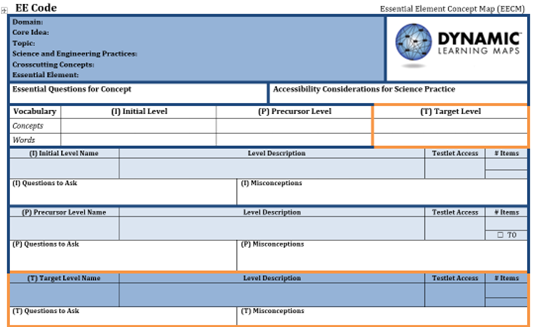
\includegraphics[width=1\linewidth]{images/fig2.png}
    \caption{Science EECM Template}
\end{figure}

At an item writer workshop, items/testlets were drafted by 49 teachers from five states. The item writers had been selected through an application process, based on their experience and expertise. Teachers were trained on the DLM assessment, characteristics of students with SCD, and principles of good item writing. Teachers used the Essential Element Concept Maps to draft testlets. Science testlets are designed to be instructionally relevant and contain an engagement activity followed by items. The engagement activity is often a story about a student who is doing a science activity, but may also be a video of a science phenomenon, or an informational text about a science concept, depending on the linkage level characteristics. The purpose of the engagement activity is to create a context for the items that follow, engage the student's interest, and activate prior knowledge. The items are intended to engage students in the science practices within the context provided by the engagement activity. Precursor linkage level and target linkage level items are multiple choice with three answer options while initial level items are teacher observations with five answer options.

The Dynamic Learning Maps test development process is designed to produce high quality measures of the identified constructs. Science testlets underwent a series of reviews, including: science content review; editorial review, internal content and special education reviews; as well as external reviews. The first two of these reviews were conducted by Dynamic Learning Maps staff. First, the science content review focused on scientific accuracy of the content, the alignment of the testlet content with the linkage level in terms of science concept and science or engineering practice, and the pedagogical relevance of the testlet engagement activity. Second, editorial review ensured consistency of testlet style across Dynamic Learning Maps Assessment System content areas that accessibility guidelines were met, and that content was accurate. The remaining two reviews were conducted by teachers from the states that participate in the DLM science alternate assessment.

The content and special education review process for science was conducted by teachers with expertise in science content, or teaching students with significant cognitive disabilities. Reviewers were experienced special education and science teachers. The reviewers completed training on the DLM assessment program and the review criteria. Content and special education review consists of criteria, such as: adherence to Dynamic Learning Maps style guidelines, quality of science content, accessibility issues, and bias concerns. Testlet content was reviewed for clear alignment with the linkage level in terms of science concept and science or engineering practice, appropriateness of the depth of knowledge classification and the complexity of the task, quality of answer options, and correctness of science content. Testlets were reviewed for compliance with accessibility criteria, which included: appropriateness of: cognitive load, text complexity, images, and alternate text for images. Bias considerations included item dependence on prior knowledge or experiences. Content and special education reviewers entered evaluative information into an online survey and/or recommended revisions to testlets. Testlets that did not meet criteria were revised.

The external review process for science was conducted by teachers with expertise in science content, or teaching students with significant cognitive disabilities. Reviewers completed applications and were selected based on expertise and experience criteria. Reviewers completed online training on the Dynamic Learning Maps program, student population, and test design criteria. Reviews were completed by a panel. Each reviewer was assigned to evaluate one specific category, either accessibility, content, or bias and sensitivity. External reviewers entered evaluative information through the computer system. Testlets and items that were flagged by external reviewers were examined by the content team for revision or rejection. Revisions were made as needed to address reviewer concerns. After quality checks were completed, testlets were ready to be used with students. 

\subsection*{Method for Research Question 3}

During the pilot test, each Essential Element and linkage level was assessed by one testlet. In total, 81 testlets were administered. Each student was administered 9 testlets at one linkage level that was chosen based on information from the student’s First Contact Survey. The system assigned each student to a specific linkage level based on teacher’s responses to the expressive communication questions about that student’s abilities. 

\begin{table}[ht]
\caption{Number of Testlets Piloted by Grade Span}
\begin{tabular}{lcccc}
\hline
Linkage Level & Elementary School & Middle School & High School & Total \\ \hline
Initial	& 9 & 9 & 9 & 27 \\
Precursor & 9 & 9 & 9 & 27 \\
Target & 9 & 9 & 9 & 27 \\
Total & 27 & 27 & 27 & 81 \\ \hline
\end{tabular}
\end{table}

Items were administered to a total of 1,606 students from four states (Table 5). The breakdown of participants by linkage level (Table 5) shows 54\% of students were at the target linkage level, 20\% of students were at the precursor linkage level, and about 26\% of students were at the initial linkage level. The number of participants by grade span shows that 36\% of students were in elementary (3rd – 5th grade), 35\% were in middle school (6th – 8th grade), 29\% were in high school (9th – 10th grade).

\begin{table}[ht]
\caption{Participants by Grade Span and Linkage Level}
\begin{tabular}{lllll}
\hline
Grade Span & Number of Students & Initial Level & Precursor Level & Target Level \\ \hline
Elementary & 575 & 155 & 131 & 289 \\
Middle & 563 & 146 & 115 & 301 \\
High School & 468 & 111 & 75 & 282 \\
Total & 1,606 & 412 & 321 & 872 \\ \hline
\end{tabular}
\end{table}

Data from the pilot were reviewed to evaluate the item quality and accessibility. The minimum sample size for the data to be considered reliable was 20 cases. The percentage of students who answered an item correctly, or p-value, was the primary review criteria. If the p-value was less than .35, the item could be too challenging because 35\% is approximately the chance of randomly selecting the correct response. Therefore, if fewer than 35\% of students responded correctly to the item, the content might be inaccessible. We examined each item that was flagged for low p-value (see Appendix A) and considered features that might make it too challenging. The percentage of students who selected other answer options was also examined to determine which other answer options were attractive to students and the cause of the attraction. 

Individual items and testlets were examined and possible causes for the flag were considered. A team of science content and special education experts conducted the review. Group consensus was used to make item-level decisions. After item-level decisions were made, testlets were evaluated to determine if the entire testlet would be retained or rejected. 

\subsection*{Results for Research Question 3}

Overall, 15\% of the items were flagged for low p-value. The flagged items were evenly spread across the grade levels (Table 6). 

\begin{table}[ht]
\caption{Flagged Items by Grade Span}
\begin{tabular}{lccc}
\hline
Grade Span & Number Of Item Flags & Total Number Of (Eligible) Items & Percent Flagged \\ \hline
Elementary & 13 & 83 & 15.7\% \\
Middle School & 12 & 83 & 14.5\% \\
High School & 13 & 85 & 15.3\% \\
Total & 38 & 251 & 15.1\% \\ \hline
\end{tabular}
\end{table}

To compare the difficulty of each linkage level, the average p-value for each Essential Element and Linkage Level was calculated (Tables 7, 8, and 9). 

\begin{table*}[thp]
\caption{Average P-value by Linkage Level and EE for Elementary}
\begin{tabular}{llccc}
\hline
& & \multicolumn{3}{c}{Linkage Level} \\ \cline{3-5}
& & Intial & Precursor & Target \\ \hline
\multirow{3}{*}{Earth \& Space Science} & SCI.EE.5.ESS1-2 & 0.4481 & \cellcolor{yellow}0.2989 & 0.7509 \\
& SCI.EE.5.ESS2-1 & 0.4599 & 0.4252 & 0.6957 \\
& SCI.EE.5.ESS3-1 & 0.4344 & \cellcolor{yellow}0.2493 & 0.5608 \\ \hline
\multirow{2}{*}{Life Science} & SCI.EE.5.LS1-1 & 0.4875 & 0.6146 & 0.4498 \\
& SCI.EE.5.LS2-1 & 0.5626 & 0.4766 & 0.5465 \\ \hline
\multirow{4}{*}{Physical Science} & SCI.EE.5.PS1-2 & 0.3937 & 0.4468 & 0.4651 \\
& SCI.EE.5.PS1-3 & 0.5186 & 0.4672 & 0.7109 \\
& SCI.EE.5.PS2-1 & 0.4795 & 0.5645 & 0.3821 \\
& SCI.EE.5.PS3-1 & 0.4817 & 0.4745 & 0.6573 \\ \hline
\end{tabular}
\textit{Note: Highlighted items represent testlets that were rejected}
\end{table*}

\begin{table*}[thp]
\caption{Average P-value by Linkage Level and EE for Middle School}
\begin{tabular}{llccc}
\hline
& & \multicolumn{3}{c}{Linkage Level} \\ \cline{3-5}
& & Intial & Precursor & Target \\ \hline
\multirow{3}{*}{Earth \& Space Science} & SCI.EE.MS.ESS2-2 & 0.4275 & 0.4649 & 0.5392 \\
 & SCI.EE.MS.ESS2-6 & 0.6856 & 0.5497 & 0.6400 \\
 & SCI.EE.MS.ESS3-3 & 0.5025 & 0.4491 & 0.5430 \\ \hline
\multirow{3}{*}{Life Science} & SCI.EE.MS.LS1-3 & 0.4987 & 0.4408 & 0.5811 \\
 & SCI.EE.MS.LS1-5 & 0.6041 & 0.5252 & 0.8476 \\
 & SCI.EE.MS.LS2-2 & 0.5112 & 0.6443 & 0.4497 \\ \hline
\multirow{3}{*}{Physical Science} & SCI.EE.MS.PS1-2 & 0.4436 & 0.4218 & 0.5147 \\
 & SCI.EE.MS.PS2-2 & \cellcolor{yellow}0.3835 & 0.4955 & 0.6018 \\
 & SCI.EE.MS.PS3-3 & 0.5187 & \cellcolor{yellow}0.2888 & 0.6363 \\ \hline
\end{tabular}
\textit{Note: Highlighted items represent testlets that were rejected}
\end{table*}

\begin{table*}[thp]
\caption{Average P-value by Linkage Level and EE for High School}
\begin{tabular}{llccc}
\hline
& & \multicolumn{3}{c}{Linkage Level} \\ \cline{3-5}
& & Intial & Precursor & Target \\ \hline
\multirow{3}{*}{Earth \& Space Science} & SCI.EE.HS.ESS1-4 & 0.5317 & 0.4242 & 0.3169 \\
 & SCI.EE.HS.ESS3-2 & 0.5789 & \cellcolor{yellow}0.2980 & 0.5469 \\
 & SCI.EE.HS.ESS3-2 & 0.8235 & 0.4286 & 0.4747 \\ \hline
\multirow{3}{*}{Life Science} & SCI.EE.HS.LS1-2 & 0.4082 & 0.5469 & 0.4262 \\
 & SCI.EE.HS.LS2-2 & 0.5064 & 0.4219 & 0.6478 \\
 & SCI.EE.HS.LS4-2 & 0.4776 & 0.5606 & 0.7666 \\ \hline
\multirow{3}{*}{Physical Science} & SCI.EE.HS.PS1-2 & 0.4401 & \cellcolor{yellow}0.2654 & 0.4967 \\
 & SCI.EE.HS.PS2-3 & 0.5104 & 0.3897 & 0.6738 \\
 & SCI.EE.HS.PS3-4 & 0.4604 & 0.4074 & 0.5538 \\ \hline
\end{tabular}
\textit{Note: Highlighted items represent testlets that were rejected}
\end{table*}

To compare the difficulty across science domains, the ranges of p-values for each of the three domains at each grade level were compared (Table 10). 

\begin{table*}[thp]
\caption{Summary of Average P-values for Each Science Domain}
\begin{tabular}{lccc}
\hline
 & \textbf{Earth \& Space Science} & \textbf{Life Science} & \textbf{Physical Science} \\ \hline
Elementary & 0.43-0.75 & 0.45-0.61 & 0.38-0.71 \\
Middle School & 0.43-0.69 & 0.44-0.84 & 0.44-0.64 \\
High School & 0.32-0.82 & 0.41-0.77 & 0.41-0.67 \\ \hline
\end{tabular}
\end{table*}

\section*{CONCLUSIONS}

\textit{Research Question 1: How can the science disciplinary core ideas, crosscutting concepts, and science and engineering practices described in A Framework for K-12 Science Education be made accessible to students with SCD?}

Through the use of the \textit{Next Generation Science Standards} and Universal Design principles, a set of alternate science content standards, called Essential Elements, was drafted. These Essential Elements make the \textit{Framework} accessible to students with SCD by providing links to grade-level science concepts that are accessible via three different linkage levels. The Essential Elements were reviewed by science content experts, special education experts, and states to ensure representation of the content of the \textit{Framework} and accessibility for students with SCD. Review feedback supported the accessibility of the Essential Elements and alignment with the \textit{Framework} dimensions. Additional evidence of the accessibility of the Essential Elements came from assessment data. 

\textit{Research Question 2: How can the new alternate standards be assessed?}

Using established procedures, test specifications were created (the Essential Element Concept Maps) and items were written. The items/testlets underwent an established, rigorous review process that allowed iterative refinements until all reliability and validity criteria were met. 

\textit{Research Question 3: How do we know the newly created alternate standards and assessments are accessible?}

Assessment data provided evidence of accessibility of alternate standards and assessments. The majority (85\%) of the items met the minimum threshold for percentage of students who answered correctly (p-value) of 35\%, which provides evidence of the accessibility of the items (and of the Essential Elements). The review of item-level and testlet-level data, as well as the internal and external reviews during the test development process, supports the claims that the science assessment items were of high quality and not too difficult. Furthermore, exceeding p-value thresholds supports that students with SCD could demonstrate understanding of science concepts. Six of 81 testlets were found to be too difficult and were rejected. The linkage levels for which testlets were rejected are highlighted in orange (Tables 7, 8,\& 9). No patterns were noted that indicated differences in accessibility by grade level; two testlets were rejected from each grade level (elementary, middle, and high school). Physical science and earth and space science testlets may have been less accessible than life science testlets because three of the rejected testlets were in physical science and three were in earth and space science, while none were in life science. The higher flag rate at the precursor level indicates that precursor linkage level testlets may have been less accessible than target and initial linkage level testlets. Five of the six rejected testlets were at the precursor linkage level and one was at the initial linkage level, while no target level testlets were rejected. 

Twenty-eight (15\%) of the assessment items were found to either be too difficult or present accessibility challenges. These 28 items were revised. One pattern that was noted was 27 of the 38 flagged items (71\% of flagged items) were at the precursor linkage level. This pattern indicates that precursor linkage level testlets might be less accessible than testlets at other linkage levels. The precursor linkage level testlets were examined to determine possible causes for the higher relative difficulty of precursor level testlets. It was noted that the linkage level descriptors at the precursor level ask students to use more complex skills, such as developing models and making evidence-based claims. When these linkage levels were assessed, success on items relied on application of a science skill and accessing facts from memory. The review team believed that precursor level testlets could be made more accessible, while still assessing the skills described by the linkage level if more context was provided to students. The provision of additional context could possibly compensate for limitations of short-term and long-term memory that are often present in students with SCD. The testlets were revised to give students context in the form of science stories that provide background information and activate prior knowledge. Items and testlets were revised and included in the fall 2015 field test. Fall 2015 field test data were not yet available at the time of this paper, but will be examined to evaluate the effect of changes to testlet design.

\subsection*{Implications}

Recent changes in science education influence what students will learn, how students will be taught, and how students will be assessed. The publication of \textit{A Framework for K-12 Science Education} (National Research Council, 2012) and the \textit{Next Generation Science Standards} (A\-chieve, 2013) have initiated major content changes that present great challenges to all science teachers (e.g. Lederman\& Lederman, 2014; Stage, Asturias, Cheuk, Daro,\& Hampton, 2013). Historically, the quality and quantity of science teaching experienced by students with SCD have been less than that experienced by their general education age peers. First, students with SCD have typically been taught a life-skills based curriculum and/or science content that is at substantially lower cognitive levels than the content taught to their age peers (Karvonen et al., 2011; Kleinert, Browder,\& Towles-Reeves, 2009).  Second, common science teaching practices that are currently used with students with SCD emphasize rote knowledge and behavioral changes instead of conceptual understanding and cognitive development. Third, most teachers of students with SCD have not had opportunities to develop skill in teaching science. The effect of current shifts in science education on special education is a dearth of curriculum and assessment tools that are: accessible to students with SCD, linked to grade-level science content, and aligned with the new science framework. However, high quality teacher resources are critical to facilitating quality science teaching for students with SCD.

The results of this study have important implications for teacher education. The finding that students with SCD can demonstrate understanding of science concepts implies that current models used to teach science to students with SCD that emphasize rote knowledge, such as task analysis and time delay, should be supplemented with models that can help students construct conceptual understanding.  However, the use of conceptual science teaching methods with students with SCD is a significant change that will require systemic supports. Furthermore, few research findings regarding teaching science for students in general education have been applied to students with SCD and there is much that we do not know about how students with SCD best learn science. More research is needed on conceptual science teaching with students with SCD.

\subsection*{Future Directions}

During the process of test development, Dynamic Learning Maps state partners raised concerns about the lack of resources to help teachers make science accessible to students with SCD. To address this concern, teachers at an item writer workshop were asked to create science instructional activities that could be used to teach the science concepts and engage students in the science or engineering practices, as specified in the Essential Element Concept Maps. It was observed that many special education teachers struggled with this exercise because they had not taught the science content before, while some science teachers struggled to meet the accessibility needs of students with SCD because they were not familiar with the students. It is clear that teachers of students with SCD have professional development needs that must be met before the capacity for teaching science can be built. This fall, the consortium reviewed and refined three model science instructional activities to support Essential Element-based instruction. These activities will be published on the Dynamic Learning Maps website next spring. Development of a full set of resources is desired, but the resources to complete this task have not yet been identified. 

\section*{ACKNOWLEDGEMENTS}
A prior version of this paper was presented at the 2016 annual meeting of The Association for Science Teacher Education, Reno, Nevada. The author would like to acknowledge the collaborative efforts of the partner states and staff that comprise the Dynamic Learning Maps Consortium in the development of the DLM Alternate Assessment System and the DLM Science Alternate Assessment. The Dynamic Learning Maps project is directed by Dr. Meagan Karvonen.

\end{large}
\clearpage
\section*{REFERENCES}\par 

\leftskip 0.25in
\parindent -0.25in 
Browder, D. M., Wakeman, S. Y., Flowers, C., Rickelman, R. J., Pugalee, D.,\& Karvonen, M. (2007). Creating access to the general curriculum with links to grade-level content for students with significant cognitive disabilities: An explication of the concept. \textit{The Journal of Special Education, 41}(1), 2–16. \url{http://doi.org/10.1177/00224669070410010101}

Browder, D. M., Wood, L., Thompson, J.,\& Ribuffo, C. (2014). Evidence-based practices for students with severe disabilities (Document No. IC-3). Retrieved from: \url{http://ceedar.education.ufl.edu/tools/innovation-configurations/}

Browder, D. M., Trela, K., Courtade, G. R., Jimenez, B. A., Knight, V.,\& Flowers, C. (2012). Teaching mathematics and science standards to students with moderate and severe developmental disabilities. \textit{The Journal of Special Education, 46}(1), 26–35. doi: 10.1177/0022466910369942

CAST, Inc. (2012). Universal Design for Learning. Retrieved from \url{http://www.udlcenter.org/aboutudl/whatisudl}

Courtade, G. R., Spooner, F.,\& Browder, D. M. (2007). Review of studies with students with significant cognitive disabilities which link to science standards. \textit{Research and Practice for Persons with Severe Disabilities, 32}(1), 43–49. doi: 10.2511/rpsd.32.1.43

Dynamic Learning Maps. (August 2013). The first contact census student characteristics. \url{http://dynamiclearningmaps.org/sites/drupal.dynamiclearningmaps.org/files/documents/First_Contact_Handout_8_6_13.pdf}

Dynamic Learning Maps. (December 2014). \textit{DLM Science 2014-16 Phase I Blueprint}. Lawrence, KS: University of Kansas. 

Dynamic Learning Maps. (June 2015). \textit{Dynamic Learning Maps Essential Elements for Science}. Lawrence, KS: University of Kansas. 

Dynamic Learning Maps. (December 2015). \textit{Summary of the Science Dynamic Learning Maps™ Alternate Assessment Development Process}. Lawrence, KS: University of KS.

Federal Register (December 9, 2003). Title I—Improving the academic achievement of the disadvantaged; final rule. Vol. 68, (236). U. S. Department of Education. Washington D.C. Retrieved from: \url{https://www2.ed.gov/legislation/FedRegister/finrule/2003-4/120903a.pdf}

Karvonen, M., Bechard, S.,\& Wells-Moreaux, S. (2015). Accessibility considerations for students with significant cognitive disabilities who take computer-based alternate assessments. Paper presented at the 2015 annual meeting of the American Educational Research Association, Chicago, IL.

Karvonen, M., Wakeman, S. Y., Browder, D. M., Rogers, M. A. S.,\& Flowers, C. (2011). \textit{Academic curriculum for students with significant cognitive disabilities: Special education teacher perspectives a decade after IDEA 1997}.

Kleinert, H. L., Browder, D. M.,\& Towles-Reeves, E. A. (2009). Models of cognition for students with significant cognitive disabilities: Implications for assessment. \textit{Review of Educational Research, 79}(1), 301–326. doi: 10.3102/0034654308326160

Individuals with Disabilities Education Improvement Act of 2004 (IDEA). Public Law 108-446. U.S. Code. 20 2004. § 1400 et seq. 

Lederman, N. G.,\& Lederman, J. S. (2014). The next generation science standards: Implications for preservice and inservice science teacher education. \textit{Journal of Science Teacher Education, 25}(2), 141–143. doi: 10.1007/s10972-014-9382-3

Miller, B. T., Krockover, G. H.,\& Doughty, T. (2013). Using iPads to teach inquiry science to students with a moderate to severe intellectual disability: A pilot study. \textit{Journal of Research in Science Teaching, 50}(8), 887–911. doi: 10.1002/tea.21091

Miller, B. T., Doughty, T.,\& Krockover, G. H. (2015). Using science inquiry methods to promote self-determination and problem-solving skills for students with moderate intellectual disability. \textit{Education and Training in Autism and Developmental Disabilities, 50}(3), 356–368.

Mislevy, R. J., Almond, R. G. and Lukas, J. F. (2003), A brief introduction to evidence-centered design. ETS Research Report Series. doi: 10.1002/j.2333-8504.2003.tb01908.x

Spooner, F., Knight, V., Browder, D. M., Jimenez, B.,\& DiBiase, W. (2011). Evaluating evidence-based practice in teaching science content to students with severe developmental disabilities. \textit{Research and Practice for Persons with Severe Disabilities, 36}(1-2), 62–75. \url{http://doi.org/10.2511/rpsd.36.1-2.62} 

Stage, E. K., Asturias, H., Cheuk, T., Daro, P. A.,\& Hampton, S. B. (2013). Opportunities and challenges in Next Generation Standards. \textit{Science, 340}, 276–277. doi: 10.4324/9780203873465

Wakeman, S. Y., Karvonen, M.,\& Ahumada, A. (2013). Changing instruction to increase achievement for students with moderate to severe intellectual disabilities. \textit{Teaching Exceptional Children, 46}(2), 6–13.

Wells-Moreaux, S., Bechard, S.,\& Karvonen, M. (2015). \textit{Accessibility manual for the Dynamic Learning Maps™ Alternate Assessment, 2015-2016}. Lawrence, KS: The University of Kansas Center for Educational Testing and Evaluation.
\clearpage
\leftskip 0in
\parindent 0in 

\begin{table*}[t]
\large \textbf{Appendix A} \normalsize
\caption*{Summary of Average Testlet Difficulty Values for Elementary}
\begin{tabular}{|l|l|l|l|l|l|}
\hline
Domain & Essential Element & LL & Number of Students & Average \textit{p}-value & Number of Items Flagged \\ \hline
\multirow{9}{*}{Earth \& Space Science} & SCI.EE.5.ESS1-2 & I & 145 & 0.4481 & 1 \\ \cline{2-6}
 & & \cellcolor{yellow}P & \cellcolor{yellow}126 & \cellcolor{yellow}0.2989 & \cellcolor{yellow}3 \\ \cline{2-6}
 & & T & 272 & 0.7509 & 0 \\ \cline{2-6}
 & SCI.EE.5.ESS2-1 & I & 142 & 0.4599 & 0 \\ \cline{2-6}
 & & P & 128 & 0.4252 & 1 \\ \cline{2-6}
 & & T & 269 & 0.6957 & 0 \\ \cline{2-6}
 & SCI.EE.5.ESS3-1 & I & 146 & 0.4344 & 0 \\ \cline{2-6}
 & & \cellcolor{yellow}P & \cellcolor{yellow}126 & \cellcolor{yellow}0.2493 & \cellcolor{yellow}3 \\ \cline{2-6}
 & & T & 263 & 0.5608 & 0 \\ \hline
\multirow{6}{*}{Life Science} & SCI.EE.5.LS1-1 & I & 147 & 0.4875 & 0 \\ \cline{2-6}
 & & P & 127 & 0.6146 & 0 \\ \cline{2-6}
 & & T & 269 & 0.4498 & 1 \\ \cline{2-6}
 & SCI.EE.5.LS2-1 & I & 147 & 0.5626 & 0 \\ \cline{2-6}
 & & P & 128 & 0.4766 & 1 \\ \cline{2-6}
 & & T & 270 & 0.5465 & 0 \\ \hline
\multirow{12}{*}{Physical Science} & SCI.EE.5.PS1-2 & I & 147 & 0.3937 & 0 \\ \cline{2-6}
 & & P & 128 & 0.4468 & 1 \\ \cline{2-6}
 & & T & 267 & 0.4651 & 0 \\ \cline{2-6}
 & SCI.EE.5.PS1-3 & I & 143 & 0.5186 & 0 \\ \cline{2-6}
 & & P & 127 & 0.4672 & 0 \\ \cline{2-6}
 & & T & 270 & 0.7109 & 0 \\ \cline{2-6}
 & SCI.EE.5.PS2-1 & I & 146 & 0.4795 & 0 \\ \cline{2-6}
 & & P & 123 & 0.5645 & 0 \\ \cline{2-6}
 & & T & 263 & 0.3821 & 2 \\ \cline{2-6}
 & SCI.EE.5.PS3-1 & I & 145 & 0.4817 & 0 \\ \cline{2-6}
 & & P & 125 & 0.4745 & 0 \\ \cline{2-6}
 & & T & 262 & 0.6573 & 0 \\ \hline
\end{tabular}
\end{table*}

\clearpage

\begin{table*}[t]
\caption*{Summary of Average Testlet Difficulty Values for Middle School}
\begin{tabular}{|l|l|l|l|l|l|}
\hline
& Essential Element & LL & Number of Students & Average \textit{p}-value & Number of Items Flagged \\ \hline
\multirow{9}{*}{Earth \& Space Science} & SCI.EE.MS.ESS2-2 & I & 135 & 0.4275 & 0 \\  \cline{2-6}
 & & P & 114 & 0.4649 & 1 \\  \cline{2-6}
 & & T & 287 & 0.5392 & 1 \\  \cline{2-6}
 & SCI.EE.MS.ESS2-6 & I & 134 & 0.6856 & 0 \\  \cline{2-6}
 & & P & 114 & 0.5497 & 0 \\  \cline{2-6}
 & & T & 299 & 0.64 & 1 \\  \cline{2-6}
 & SCI.EE.MS.ESS3-3 & I & 134 & 0.5025 & 0 \\  \cline{2-6}
 & & P & 111 & 0.4491 & 1 \\  \cline{2-6}
 & & T & 296 & 0.543 & 0 \\  \hline
\multirow{9}{*}{Life Science} & SCI.EE.MS.LS1-3 & I & 132 & 0.4987 & 0 \\ \cline{2-6}
 & & P & 111 & 0.4408 & 1 \\  \cline{2-6}
 & & T & 300 & 0.5811 & 0 \\  \cline{2-6}
 & SCI.EE.MS.LS1-5 & I & 132 & 0.6041 & 0 \\  \cline{2-6}
 & & P & 114 & 0.5252 & 1 \\  \cline{2-6}
 & & T & 291 & 0.8476 & 0 \\  \cline{2-6}
 & SCI.EE.MS.LS2-2 & I & 134 & 0.5112 & 0 \\  \cline{2-6}
 & & P & 115 & 0.6443 & 1 \\  \cline{2-6}
 & & T & 293 & 0.4497 & 0 \\  \hline
\multirow{9}{*}{Physical Science} & SCI.EE.MS.PS1-2 & I & 136 & 0.4436 & 0 \\ \cline{2-6}
 & & P & 113 & 0.4218 & 1 \\  \cline{2-6}
 & & T & 293 & 0.5147 & 0 \\  \cline{2-6}
 & SCI.EE.MS.PS2-2 & \cellcolor{yellow}I & \cellcolor{yellow}133 & \cellcolor{yellow}0.3835 & \cellcolor{yellow}1 \\  \cline{2-6}
 & & P & 111 & 0.4955 & 0 \\  \cline{2-6}
 & & T & 290 & 0.6018 & 0 \\  \cline{2-6}
 & SCI.EE.MS.PS3-3 & I & 133 & 0.5187 & 0 \\  \cline{2-6}
 & & \cellcolor{yellow}P & \cellcolor{yellow}110 & \cellcolor{yellow}0.2888 & \cellcolor{yellow}3 \\  \cline{2-6}
 & & T & 298 & 0.6363 & 0 \\ \hline
\end{tabular}
\end{table*}

\clearpage

\begin{table*}[t]
\caption*{Summary of Average Testlet Difficulty Values for High School}
\begin{tabular}{|l|l|l|l|l|l|}
\hline
& Essential Element & LL & Number of Students & Average \textit{p}-value & Number of Items Flagged \\ \cline{2-6}
\multirow{9}{*}{Earth \& Space Science} & SCI.EE.HS.ESS1-4 & I & 101 & 0.5317 & 0 \\ \cline{2-6}
 & & P & 66 & 0.4242 & 0 \\ \cline{2-6}
 & & T & 243 & 0.3169 & 2 \\ \cline{2-6}
 & SCI.EE.HS.ESS3-2 & I & 95 & 0.5789 & 0 \\ \cline{2-6}
 & & \cellcolor{yellow}P & \cellcolor{yellow}66 & \cellcolor{yellow}0.298 & \cellcolor{yellow}2 \\ \cline{2-6}
 & & T & 245 & 0.5469 & 1 \\ \cline{2-6}
 & SCI.EE.HS.ESS3-2 & T & 253 & 0.8235 & 0 \\ \cline{2-6}
 & & I & 98 & 0.4286 & 0 \\ \cline{2-6}
 & & P & 66 & 0.4747 & 0 \\ \hline
\multirow{9}{*}{Life Science} & SCI.EE.HS.LS1-2 & I & 98 & 0.4082 & 0 \\ \cline{2-6}
 & & P & 64 & 0.5469 & 1 \\ \cline{2-6}
 & & T & 264 & 0.4262 & 1 \\ \cline{2-6}
 & SCI.EE.HS.LS2-2 & I & 104 & 0.5064 & 0 \\ \cline{2-6}
 & & P & 64 & 0.4219 & 0 \\ \cline{2-6}
 & & T & 266 & 0.6478 & 0 \\ \cline{2-6}
 & SCI.EE.HS.LS4-2 & I & 104 & 0.4776 & 0 \\ \cline{2-6}
 & & P & 66 & 0.5606 & 0 \\ \cline{2-6}
 & & T & 262 & 0.7666 & 0 \\ \hline
\multirow{9}{*}{Physical Science} & SCI.EE.HS.PS1-2 & I & 104 & 0.4401 & 0 \\ \cline{2-6}
 & & \cellcolor{yellow}P & \cellcolor{yellow}65 & \cellcolor{yellow}0.2654 & \cellcolor{yellow}3 \\ \cline{2-6}
 & & T & 251 & 0.4967 & 0 \\ \cline{2-6}
 & SCI.EE.HS.PS2-3 & I & 97 & 0.5104 & 0 \\ \cline{2-6}
 & & P & 65 & 0.3897 & 1 \\ \cline{2-6}
 & & T & 249 & 0.6738 & 0 \\ \cline{2-6}
 & SCI.EE.HS.PS3-4 & I & 98 & 0.4604 & 0 \\ \cline{2-6}
 & & P & 63 & 0.4074 & 2 \\ \cline{2-6}
 & & T & 251 & 0.5538 & 0 \\ \hline
\end{tabular}
\end{table*}

\end{document}
